\documentclass[a4paper,oneside,12pt]{report}

\usepackage[utf8]{inputenc}
\usepackage[T1]{fontenc}
\usepackage[french]{babel}
\usepackage{hyperref}
\usepackage{fancyhdr}
\usepackage[official]{eurosym}
\usepackage{stageutc}

\newcommand{\cf}[1]{cf. #1}
\newcommand{\etranger}[1]{\textit{#1}}

\newcommand{\refsection}[1]{section~\ref{section:#1}}
\newcommand{\cfsection}[1]{\cf{\refsection{#1}}}

\newcommand{\reffigure}[1]{figure~\ref{figure:#1}}
\newcommand{\cffigure}[1]{\cf{\reffigure{#1}}}


\newcommand{\acentreon}{Centreon}
\newcommand{\alinotp}{LinOTP}
\newcommand{\aintranet}{Intranet}
\newcommand{\atypo}{Typo3}
\newcommand{\aad}{Microsoft Active Directory}
\newcommand{\aradius}{RADIUS}
\newcommand{\afreerad}{FreeRADIUS}

\newcommand{\asmile}{Smile}
\newcommand{\abusys}{BU Système}
\newcommand{\abugan}{BU Ganesh}
\newcommand{\alse}{LSE}

\newcommand{\ame}{Jérémy Subtil}
\newcommand{\apakou}{Patrick Kouassi}
\newcommand{\asuiveur}{Dritan Nace}
\newcommand{\amabes}{Maxime Besson}
\newcommand{\agulet}{Guilhem Lettron}
\newcommand{\asegir}{Sébastien Giraud}
\newcommand{\amimiette}{Philippe Mimiette}
\newcommand{\ahbt}{Hervé Brassart}
\newcommand{\arolel}{Romain Leleu}



\title{TN10 -- Rapport de stage}
\subtitle{Ingénieur système et développement en environnement open source}
\author{\ame}
\date{Semestre~P11}
\keywords{open source, qualité logicielle, intégration continue, système, OTP, authentification, sécurité, supervision}

\makeatletter
\hypersetup{
	pdftitle={\@title},
	pdfauthor={\@author},
	pdfsubject={\@subtitle},
	pdfkeywords={\@keywords}
}
\makeatother

\graphicspath{{figs/}}

\geometry{headheight=15pt} % for fancyhdr


\begin{document}

\maketitle

\section*{Remerciements}

Je souhaite remercier \apakou, directeur de la \abusys, qui m'a accueilli dans son équipe chez \asmile{} et qui a suivi mon évolution au cours de ces six mois de stage.

Je remercie également mon maître de stage \agulet, ingénieur système, pour m'avoir guidé tout au
long du stage, m'avoir appris un tas de choses et m'avoir payé quelques verres.

Je voudrais aussi exprimer ma gratitude envers \amabes, expert technique système, qui m'a toujours accordé du temps pour répondre à mes questions.

Je remercie également \asuiveur, mon tuteur de stage de l'UTC, pour son soutien.

Enfin, je souhaiterais exprimer mes remerciements envers tous mes collègues titulaires et bizus\footnote{C'est ainsi que l'on surnomme les stagiaires dans la \abusys.} qui m'ont tous toujours bien accueilli parmi eux et avec qui j'ai passé d'excellents moments.


\newpage

\tableofcontents
\listoffigures
\newpage

\section*{Résumé technique}

TODO


\newpage

% fancyhdr
\pagestyle{fancy}
\lhead{}

\chapter{Présentation de l'entreprise}

\section{Le groupe \asmile}

\paragraph{}
\asmile{} est une Société de Services en Ingénierie Informatique (SSII) française, dont l'activité principale repose sur le développement web et l'intégration de solutions open source\footnote{La désignation open source s'applique aux logiciels dont la licence respecte des critères précisément établis par l'Open Source Initiative, c'est-à-dire la possibilité de libre redistribution, d'accès au code source et aux travaux dérivés.~\cite{opensource}}.
\asmile{} est d'ailleurs aujourd'hui considérée comme le leader français dans le domaine.

\paragraph{}
La société a été créée en 1991 par quatre fondateurs : Jérôme Prompsy, Patrice Bertrand, Alain Arditi et Cyrille Chignardet.
\asmile{} innove alors dans le domaine des logiciels décisionnels en s'appuyant sur les méthodes de développement RAD (\textit{Rapid Application Development}).
En 1995, l'entreprise prend une nouvelle orientation du fait de la démocratisation d'Internet et des applications web.
Pionnière sur le secteur, \asmile{} se fait notamment connaître par la conception du premier site bancaire sur le web pour le Crédit Lyonnais.

\paragraph{}
En 2001, \asmile{} fait un nouveau choix stratégique en se positionnant sur les technologies open source.
En effet, en 2004, de plus en plus d'entreprises adoptent ce type de solutions qui deviennent populaires.
En 2011, \asmile{} est présent sur plusieurs gammes de produits web tels que les CMS, les portails, l'e-commerce, le décisionnel, l'ERP et l'infrastructure.
En outre, \asmile{} compte de nouveaux secteurs d'activités plus ou moins liés à l'activité du développement web : une agence média, un pôle d'exploitation, un pôle maintenance et un pôle système.

\paragraph{}
Forte de 20 ans d'expérience, \asmile{} a su se développer dans des grandes villes en métropole telles que Lyon, Bordeaux, Montpellier et Nantes.
Actuellement, le groupe continue son expansion en ouvrant d'autres agences à Aix-en-Provence, Poitiers, Grenoble et Lille.
Par ailleurs, \asmile{} manifeste aussi sa présence en Europe, avec les agences de Barcelone, Genève et Amsterdam.
Aujourd'hui, \asmile{} se développe même en dehors de l'Union Européenne, grâce aux agences de Casablanca au Maroc et de Kiev en Ukraine.

L'ensemble de ces sites sont localisés sur la \reffigure{presentation:carte}.

\begin{figure}
	\centering
	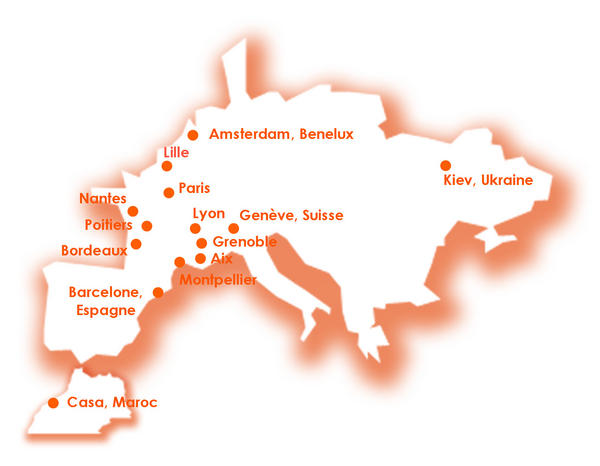
\includegraphics[width=10cm]{presentation/carte-europe-smile}
	\caption{\asmile{} en Europe}
	\label{figure:presentation:carte}
\end{figure}


\paragraph{}
Par ailleurs, l'organisation de \asmile{}, représentée en \reffigure{presentation:organigramme}, est la suivante :

\begin{itemize}
	\item en cyan, la Direction ;
	\item en beige, les BU\footnote{\textit{Business Unit}} de développement web, soit quatre unités sur Paris et quatre réparties en agences en province ;
	\item en bleu, les BU de développement européennes et offshore, qui mènent des projets locaux et des projets expertisés par Paris ;
	\item en vert, les agences métier qui regroupent les offres système, médias ainsi que les formations clients ;
	\item en violet, la BU Consulting qui gère les projets décisionnels et organisationnels.
\end{itemize}

\begin{figure}
	\centering
	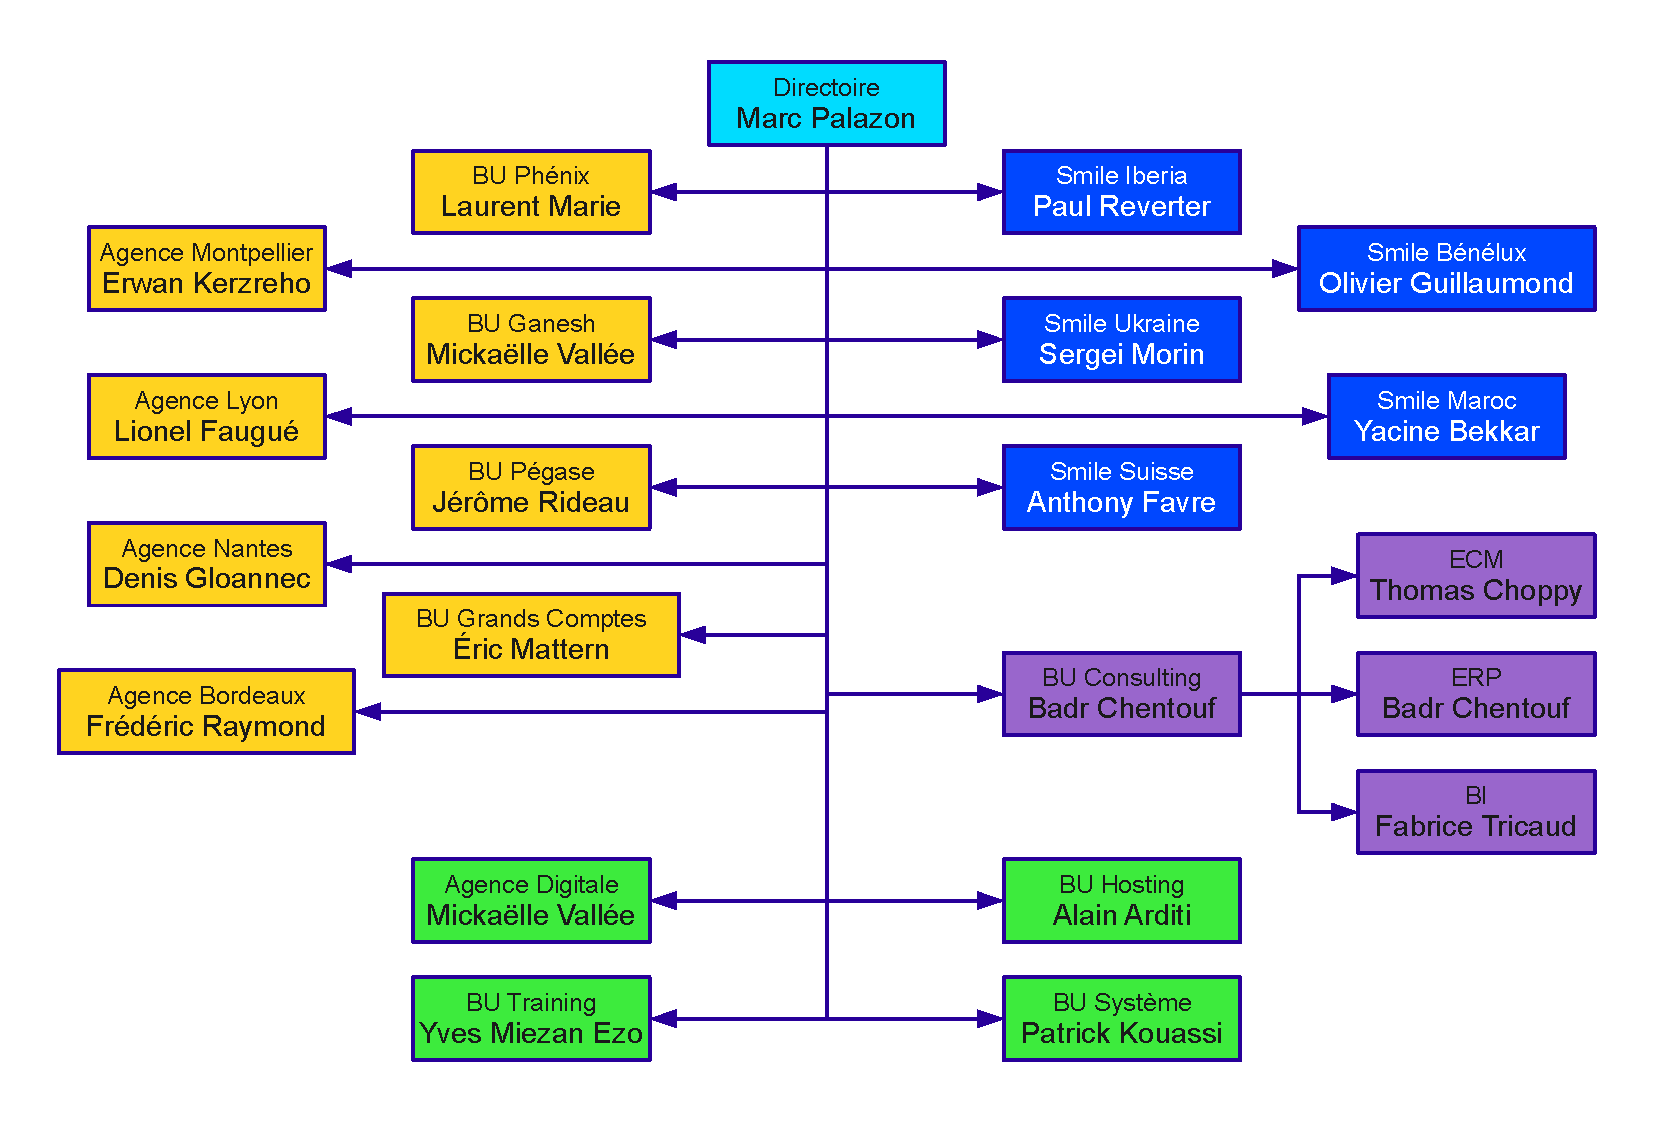
\includegraphics[width=12cm]{presentation/organigramme}
	\caption{Organigramme du groupe \asmile}
	\label{figure:presentation:organigramme}
\end{figure}


\section{Le site parisien}

\paragraph{}
Le site parisien de \asmile{} se situe à Levallois-Perret.
Il est composé de deux bâtiments : l'un est l'ancien bâtiment de Hertford British Hospital, et l'autre un building situé à 300 mètres.
Ces bâtiments accueillent aujourd'hui plusieurs pôles de \asmile{}.

\paragraph{}
Le premier ensemble consiste en le siège social et une partie de l'administration de l'entreprise :

\begin{itemize}
	\item le bureau du Président Directeur Général, Marc Palazon ;
	\item le bureau du Directeur Général, Patrice Bertrand ;
	\item le service des Relations Humaines ;
	\item le service de la communication ;
	\item les services commerciaux ;
	\item le service financier,
	\item le système interne.
\end{itemize}

\paragraph{}
Le second regroupe des équipes métier et développement, qui sont regroupées par clients et technologies maîtrisées :

\begin{description}
	\item[la \abugan{} :] spécialiste PHP, e-commerce avec Magento, expertise CMS avec eZpublish, \atypo{}, Drupal ;
	\item[la BU Pégase :] spécialiste PHP également, e-commerce avec Magento, développement spécifique avec le framework Symfony ;
	\item[la BU Phoenix :] développements spécifiques en Java, CMS avec Jahia ;
	\item[la BU Consulting :] BI, GED, ECM, ERP ;
	\item[la BU Training :] formations ;
	\item[la \abusys{} :] c'est dans cette structure que j'ai pu travailler.
\end{description}


\section{La \abusys{}}

\paragraph{}
La \abusys{} est un pôle de prestation et de conseil dans le domaine des infrastructures système et réseau.
Le rôle de cette équipe est d'accompagner les clients dans le renouvellement et l'optimisation de leurs installations.

\paragraph{}
Pour cela, l'offre système s'articule autour de quatre solutions :

\begin{itemize}
	\item l'aide au management :
	\begin{itemize}
		\item pour les plateformes web ;
		\item pour les infrastructures réseau ;
	\end{itemize}
	\item l'optimisation des infrastructures :
	\begin{itemize}
		\item par mutualisation des ressources grâces à des technologies de virtualisation ;
		\item par des réglages fins des outils suite à des tests de charge ;
	\end{itemize}
	\item la sécurité et gestion des accès utilisateurs :
	\begin{itemize}
		\item authentification ;
		\item VPN ;
		\item firewalls ;
	\end{itemize}
	\item l'étude de solutions haute disponibilité ;
	\item la migration vers des solutions open source :
	\begin{itemize}
		\item re-packaging de distributions Linux ;
		\item solutions de messageries et groupeware ;
		\item VoIP ;
		\item plate-formes d'intégration continue\ldots
	\end{itemize}
\end{itemize}

\paragraph{}
Aussi, la \abusys{} propose une offre interne de support projet pour les autres BU et agences de
\asmile{} :

\begin{itemize}
	\item le déploiement d'environnements de recette pour les projets de développement ;
	\item l'intégration des infrastructures évoluées, comme la haute disponibilité par exemple ;
	\item le soutien aux projets au niveau système.
\end{itemize}

\paragraph{}
Finalement, pour chaque besoin de l'entreprise, la \abusys{} peut proposer une solution open source adaptée.
L'offre système est illustrée en \reffigure{presentation:offre-sys}.

\begin{figure}
	\centering
	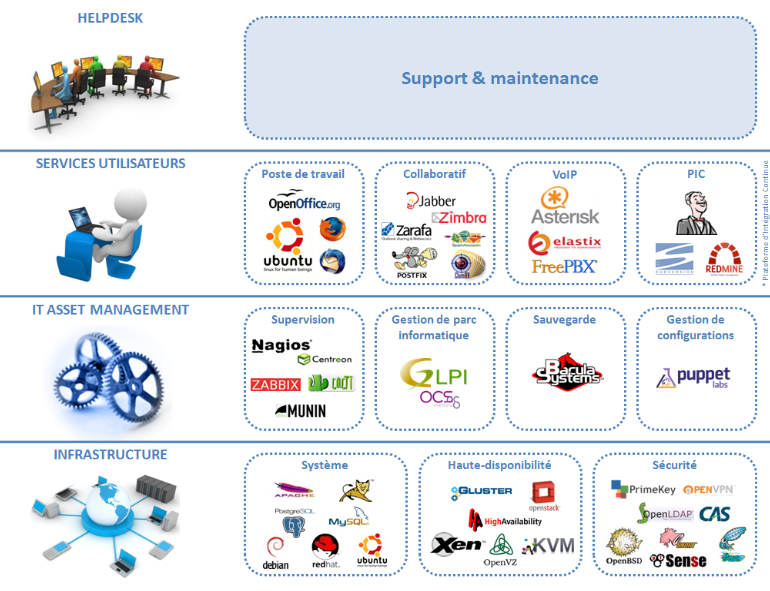
\includegraphics[width=12cm]{presentation/offre-sys}
	\caption{L'offre de la \abusys}
	\label{figure:presentation:offre-sys}
\end{figure}


\chapter{Déroulement du stage}

\section{Ma place au sein de la \abusys}

\paragraph{}
Passionné par l'écosystème de l'open source, c'est naturellement que j'ai choisi de postuler chez \asmile{} pour effectuer mon projet de fin d'études.
Sortant de la filière SRI de l'UTC, j'étais très intéressé de développer mes compétences système et c'est ainsi que j'ai pu intégrer la \abusys{}.

\paragraph{}
Dès mon premier entretien, j'ai défini avec \agulet{}, mon futur tuteur dans l'entreprise, le sujet principal de mon stage : nous avons choisi que je travaille sur les problématiques d'intégration continue.
En effet, à la \abusys{}, c'est une des spécialités de \agulet{}.
Il en est le référent quand il s'agit de fournir une prestation autour de ce domaine pour le compte de clients.
Pour ma part, c'est un sujet qui m'enthousiasme car il fait à la fois intervenir des connaissances en système et en qualité logicielle.
Ainsi, mon travail et ma réflexion sur l'intégration continue et ses outils sont développés dans le \refchap{pic}.

\paragraph{}
Par ailleurs, j'ai eu l'opportunité de travailler de bout en bout sur la mise en place d'une solution d'authentification open source particulière chez un client : \alinotp.
Elle fait intervenir les OTP, ou \etranger{One-Time Passwords}, qui sont en réalité des mots de passe éphémères générés par un matériel tiers.

Cette mission s'est déroulée sur la fin de mon stage, et j'ai alors eu l'opportunité de réaliser un véritable travail d'ingénieur système au même titre que mes collègues titulaires.
Elle est décrite en détail dans le  \refchap{linotp}.

\paragraph{}
En outre, j'ai eu l'occasion de travailler sur une multitude d'autres projets de taille plus ou moins importante :

\begin{itemize}
	\item mettre en place chez un client une solution de supervision \acentreon{} (\cfchap{centreon}) ;
	\item apporter un support d'administration système dit \emph{support projet} aux projets des différentes BU de développement de \asmile{} (\cfchap{support}) ;
	\item apporter un soutien au développement d'un projet client en retard pour \abt{} (développement avec le framework PHP Symfony et le framework JavaScript ExtJS) ;
	\item mettre en place une plateforme web de visioconférence pour \asmile{} avec la solution libre BigBlueButton ;
	\item auditer le code du logiciel libre Linbox-Converter pour le compte de Renault, qui permet de convertir des documents Microsoft Office vers d'autres formats ;
	\item chiffrer des projets système dans le cadre des processus d'avant-vente de \asmile.
\end{itemize}

\paragraph{}
Enfin, j'ai pu commencer certains travaux qui n'ont pas pu aboutir pour diverses raisons.
Ceux-ci sont décrits brièvement en \refsection{avortes}.



\section{Projets avortés}
\label{section:avortes}

TODO



\section{Planning effectif}

\paragraph{Février}
\begin{itemize}
	\item Support projet
	\item Mise en place d'un serveur de base de données Oracle
	\item Auto-formation sur la réplication de bases de données MySQL
	\item Auto-formation sur les outils Hudson/Jenkins et Selenium
	\item Travail sur l'offre \og Plateformes d'intégration continue \fg{} (PIC)
\end{itemize}

\paragraph{Mars}
\begin{itemize}
	\item Support projet
	\item Tentative de mise en place d'OpenMCU en interne
	\item Auto-formation sur l'ESB \apetals{}
	\item Développement sur le projet Abitbol
\end{itemize}

\paragraph{Avril}
\begin{itemize}
	\item Support projet
	\item Développement sur le projet Abitbol
	\item Développement Redmine
	\item Audit de code Linbox-Converter pour Renault
	\item Projet \acentreon{} pour \adacast{}
	\item Travail sur l'offre PIC
\end{itemize}

\paragraph{Mai}
\begin{itemize}
	\item Support projet
	\item Mise en place de BigBlueButton en interne
	\item Projet LinOTP pour la CNIL
	\item Travail sur l'offre PIC
\end{itemize}

\paragraph{Juin}
\begin{itemize}
	\item Support projet
	\item Fin du projet LinOTP pour la CNIL
	\item Rédaction d'une ébauche de livre blanc sur l'offre PIC
	\item Soutien au développement du projet de développement pour \abt{}
\end{itemize}

\paragraph{Juillet}
\begin{itemize}
	\item Soutien au développement du projet de développement pour \abt{}
\end{itemize}


\section{L'offre \og plateformes d'intégration continue \fg}
\label{section:pic}

\paragraph{}
Quand on sait que 70\% des projets informatiques ne respectent pas le planning initial ou se transforment en échecs~\cite{echec}, on cherche par tous les moyens à réduire les facteurs responsables.
Le manque de qualité logicielle et de suivi de projet en font évidemment parti.
Alors que ces domaines étaient encore un marché de niche il y a quelques temps de cela, aujourd'hui, de plus en plus de clients et de DSI\footnote{Directions de Services Informatiques} commencent à s'en préoccuper et à remettre en cause les méthodes classiques de gestion de projets informatiques.
C'est aussi l'occasion de tenter de pérenniser les développements qui au fil du temps perdent toujours plus en maintenabilité.

\paragraph{}
La qualité logicielle et le suivi de projets informatiques deviennent donc un véritable enjeu actuel.
Les entreprises doivent alors se doter de nouveaux process et de nouveaux outils. 
Elles peuvent les acquérir en faisant notamment appel à des prestations de conseil dans le domaine, qui font entre autres intervenir des notions de gestion de projet et de bonnes pratiques en terme de génie logiciel.
Au-delà de ça, les nouveaux outils doivent être mis en place et intégrés aux infrastructures systèmes existantes.

\paragraph{}
C'est ainsi que la \abusys{} de \asmile, sous l'impulsion de \agulet, s'est positionnée sur ce marché.
Une offre open source a été construite pour répondre au besoin de A à Z, de l'installation des outils au conseil sur leur utilisation, en passant par leur configuration personnalisée.



\subsection{Intérêt des méthodes agiles}



\subsection{La gestion de projet agile}

\subsubsection{Outil : Redmine}

\subsubsection{Outil : JIRA}

\subsubsection{Mission : Formation JIRA chez Rexel}

\subsubsection{Mission : Développement Redmine}

- Développement de plugins

- Contribution au core



\subsection{Gestion de versions du code source}

\subsubsection{Outil : Subversion}

\subsubsection{Outil : Git}

\subsubsection{Mission : Formation Subversion chez Rexel}

\subsubsection{Mission : Synchronisation de mirroirs SVN pour Rexel}

\subsubsection{Mission : Plan de formation Git}



\subsection{Tests des applications}

\subsubsection{Tests unitaires}

\subsubsection{Tests fonctionnels}

\subsubsection{Outil : Selenium}

\subsubsection{Mission : Formation Selenium chez Spir}



\subsection{Intégration continue}

\subsubsection{Outil : Hudson/Jenkins}

\subsubsection{Mission : paramétrage de la PIC de Spir}

\subsubsection{Mission : Formation Jenkins chez Spir}


\chapter{Mise en place d'une solution \alinotp{}}
\label{section:linotp}

\section{Principe des \etranger{One-Time Passwords} (OTP)}

\paragraph{}
Les \etranger{One-Time Passwords}, aussi appelés OTP, sont des mots de passe générés à un instant donné, valides pendant une courte durée et utilisables une seule fois.
La génération s'effectue grâce à des matériels adaptés, comme les tokens (\cffigure{linotp:token}) ou même des smartphones.

\begin{figure}
	\centering
	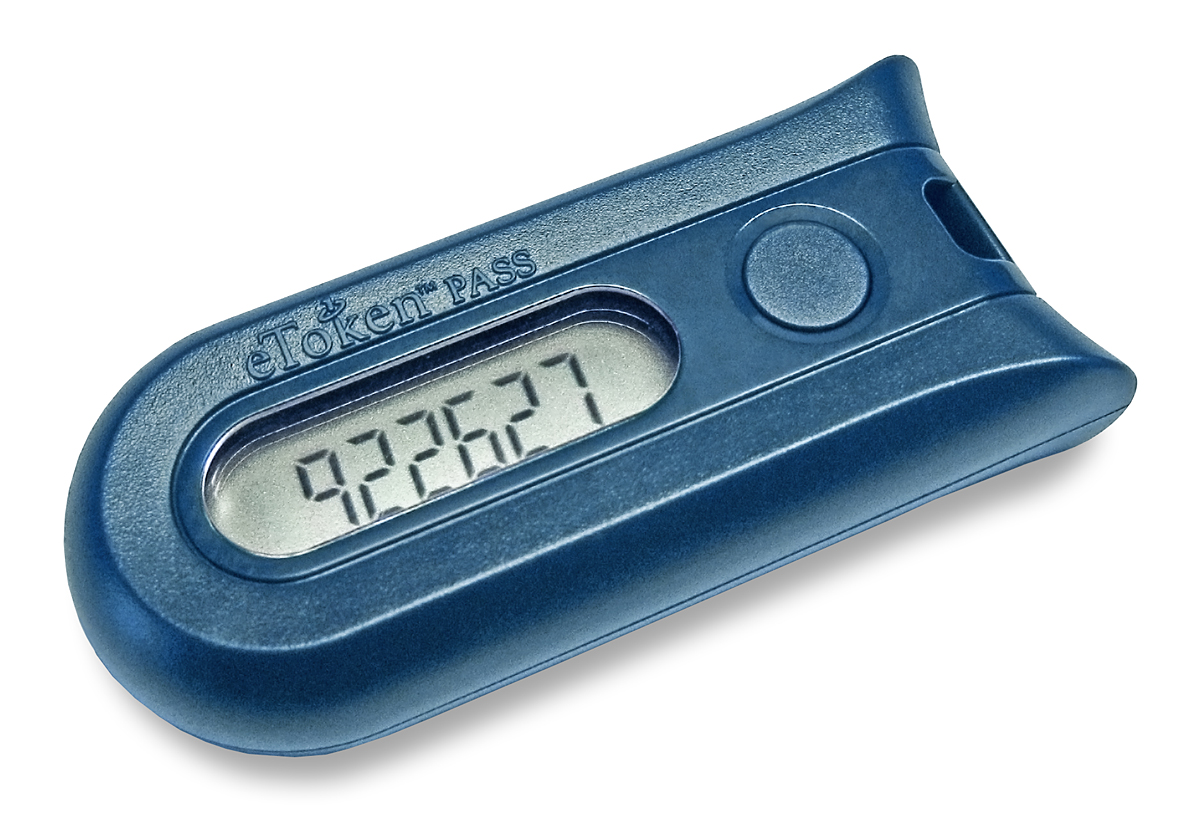
\includegraphics[width=6cm]{linotp/etoken_pass}
	\caption{Token Aladdin eToken-PASS}
	\label{figure:linotp:token}
\end{figure}

\paragraph{}
En pratique, l'utilisateur final s'authentifie en précisant son identifiant, son PIN -- qui correspond à un mot de passe statique qu'il doit mémoriser -- et l'OTP obtenu grâce au matériel.
C'est en ce sens qu'on peut parler de système à deux facteurs d'authentification (\etranger{two-factor authentication}) car on se base sur quelque chose que l'on connaît -- le PIN -- et quelque chose que l'on possède -- le token ou le smartphone.

\paragraph{}
Ainsi, l'OTP permet de résoudre un certain nombre de problèmes inhérents à l'utilisation de mots de passe statiques classiques :

\begin{itemize}
	\item on n'est plus soumis aux limites du facteur humain, qui implique souvent des compromis sur la complexité du mot de passe, et l'irrégularité de son changement ;
	\item en particulier les attaques par dictionnaire deviennent inefficaces ;
	\item les attaques par brute-force sont également limitées car elles ne peuvent plus se baser que sur des essais aléatoires dans un grand espace de clés ;
	\item la récupération silencieuse du mot de passe (via l'écoute réseau, l'installation d'un mouchard, ou l'ingénierie sociale) ne suffit plus à s'authentifier.
\end{itemize}

\paragraph{}
Par ailleurs, une méthode de génération d'OTP se base sur la synchronisation temporelle : les tokens et le serveur d'authentification OTP sont réglés à la même heure.
De plus, pour chaque token est définie une clé secrète que l'on enregistre dans la base du serveur.
C'est la combinaison de ces deux paramètres qui permet une génération et une validation des OTP.


\section{Contexte de la mission}

\paragraph{}
Au courant de l'année 2010, la Commission nationale de l'informatique et des libertés\footnote{La CNIL est une autorité administrative indépendante française. Elle est chargée de veiller à ce que l'informatique soit au service du citoyen et qu'elle ne porte atteinte ni à l'identité humaine, ni aux droits de l'homme, ni à la vie privée, ni aux libertés individuelles ou publiques.~\cite{cnil}} (CNIL) décide d'ouvrir son portail \aintranet{} confidentiel sur l'\ainternet{} pour certains de ses utilisateurs : les commissaires.
Au nombre d'une vingtaine, ceux-ci ont besoin d'accéder au contenu du site web à l'extérieur de leur lieu de travail -- à la maison par exemple.

\paragraph{}
La CNIL avait déjà fait appel aux prestations de \asmile{} pour bénéficier d'un support ponctuel sur des développements \atypo{}\footnote{\atypo{} est un système de gestion de contenu libre écrit en PHP. Fourni de base avec un certain nombre de fonctionnalités, il peut être étendu de manière impressionnante grâce à un puissant moteur de plugins. Une console d'administration permet aux auteurs et aux administrateurs de gérer facilement le contenu du site web.}, le système de gestion de contenu utilisé pour le portail.
C'est pour cela qu'elle a également choisi \asmile{} pour mettre en place l'architecture permettant un tel accès depuis l'extérieur.

\paragraph{}
C'est la CNIL elle-même qui a choisi le type d'authentification à utiliser : les OTP.
\asmile{} a alors proposé fin 2010 l'utilisation d'une solution de la marque RSA, leader sur ce marché.
Pour des raisons qui sont restées inconnues -- le nombre de licences commandées était trop faible ? -- RSA n'a pas daigné répondre aux commandes de licences et de matériel réalisées par \asmile.

Le retard sur la mise en place de l'architecture a alors poussé \asmile{} à changer de solution pour se tourner vers une alternative open source : \alinotp{}.


\section{La solution \alinotp{}}

\paragraph{}
La solution \alinotp{} se place au centre du mécanisme d'authentification :

\begin{itemize}
	\item l'interface de connexion utilisateur du portail demande à \alinotp{} de valider ou non l'authentification ;
	\item \alinotp{} consulte une base de données des utilisateurs déjà existante (e.g. un LDAP) ;
	\item les informations concernant les matériels OTP sont stockées dans sa propre base de données.
\end{itemize}

\paragraph{}
D'un point de vue technique, \alinotp{} est un serveur écrit en langage Python, avec lequel on communique par de simples requêtes HTTP.
Il est donc possible de l'administrer via d'autres outils que ceux fournis dans la distribution.
On peut imaginer développer une interface web spécifique que l'on inclurait dans une section privilégiée d'un Intranet par exemple.

\paragraph{}
Par ailleurs, \alinotp{} se décline en deux éditions :

\begin{itemize}
	\item l'édition Community, libre et gratuite, qui propose des fonctions de base pour mettre en place une maquette ;
	\item l'édition Enterprise, pour laquelle il faut acheter des licences en fonction du nombre de tokens utilisés, propose un vraie solution pour des besoins d'entreprise, avec notamment le support LDAP, \aad{}, SQL ou encore \afreerad{}.
\end{itemize}

\paragraph{}
La \reffigure{linotp:linotp-archi} illustre l'architecture modulaire de \alinotp{}~2 tout en mettant en évidence les possibilités de la solution :

\begin{itemize}
	\item en rouge est représenté le c\oe ur de \alinotp{} -- le serveur ainsi que sa base de tokens stockée dans une base de données externe ;
	\item en vert, on retrouve les différentes interfaces de résolution des utilisateurs ;
	\item en jaune, les interfaces d'authentification seront contactées par les pro\-gram\-mes clients de la solution qui demanderont si un couple identifiant~/~mot de passe OTP est bien valide ;
	\item enfin, en bleu on retrouve les différentes interfaces qui permettent d'administrer \alinotp{}, que ce soit par le web ou en ligne de commande.
\end{itemize}

\begin{figure}
	\centering
	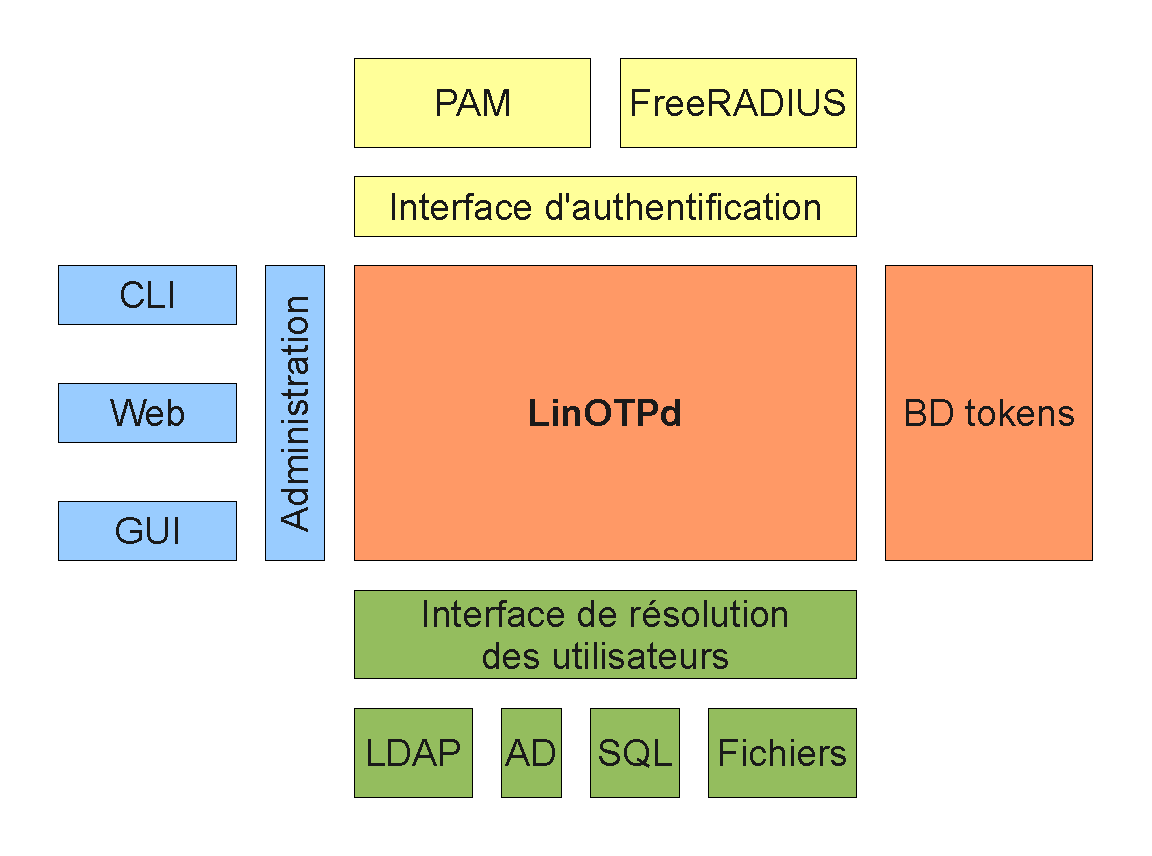
\includegraphics[width=10cm]{linotp/linotp-archi}
	\caption{Architecture modulaire de \alinotp{}~2}
	\label{figure:linotp:linotp-archi}
\end{figure}


\section{Ma démarche}

\paragraph{Mise en place d'un prototype}
C'est mon manager \apakou{} qui m'a confié la responsabilité de mettre en place la solution \alinotp{} chez notre client.

Après m'avoir présenté le contexte de la mission ainsi que le principe des OTP, il m'a demandé de mettre en place une première maquette fonctionnelle du système.
Les détails techniques de ce prototype seront décrits dans la \refsection{linotp:prototype}.

\paragraph{Présentation du prototype}
J'ai pu alors présenter ma maquette à deux reprises.

La première fois, je me suis rendu avec \asegir{}, le chef de projet de la mission, dans les bureaux de la \abugan.
En effet, ses développeurs sont responsables de la partie concernant l'adaptation du portail \atypo{} de la CNIL pour cette mission.
Grâce à ma démonstration du prototype, ils ont donc bien pu comprendre comment l'authentification OTP allait se dérouler pour les utilisateurs finaux.
Ils ont également pu obtenir les détails techniques concernant les flux de données que \atypo{} recevra de \alinotp{} et qu'ils devront traiter.

La seconde fois, nous nous sommes rendus, \apakou, \asegir{} et moi, dans les locaux du client pour faire valider mon travail par nos deux interlocuteurs : \ahbt, chef du service informatique de la CNIL, et \amimiette, un administrateur système.
Pour l'occasion, j'ai présenté un diaporama récapitulant le fonctionnement de la solution du point de vue de l'utilisateur final et décrivant techniquement via des diagrammes quelle allait être l'architecture à mettre en place, avec ses pré-requis.
J'ai pu terminer avec une démonstration du système via mon prototype.

\paragraph{Contact avec l'éditeur}
Une fois mon prototype validé, j'ai contacté directement l'éditeur \alse{} pour passer la commande de 30 tokens ainsi que des 30 licences \alinotp{} Enterprise correspondantes.
En effet, la version Enterprise est nécessaire du fait que les utilisateurs sont résolus depuis un annuaire \aad{} et que l'authentification doit se faire via un serveur \aradius.

J'en ai profité pour leur demander des conseils sur les différentes briques logicielles à utiliser sur l'architecture finale.
Par la suite, j'ai également pu leur faire de nombreux retours sur les problèmes que j'ai rencontré et sur la façon dont j'ai pu les contourner.
Cette échange donnant-donnant a été très bénéfique et présage un futur partenariat privilégié entre \asmile{} et \alse{}.

\paragraph{Mise en place de l'architecture finale}
Les détails techniques de l'architecture finale seront décrits dans la \refsection{linotp:archi-finale}.

J'ai commencé par mettre en place le système sur des environnements virtuels hébergés sur des serveurs de \asmile{}.
Cela m'a permis d'être rapidement confronté aux premiers problèmes et de les résoudre avant d'intervenir chez le client.

Une fois ma maquette jugée satisfaisante et répondant au besoin, j'ai pris rendez-vous avec le client pour mon intervention.
J'ai alors travaillé avec \amimiette{} qui m'a expliqué comment m'intégrer efficacement à leur infrastructure système existante.
Cette première intervention a duré deux jours.
En outre, j'ai pris des notes relatives à mon travail sur leurs serveurs au fur et à mesure afin de pouvoir par la suite rédiger une documentation technique complète.

Aussi, j'ai dû rapidement intervenir une seconde fois afin de corriger un premier bug découvert : l'authentification d'un utilisateur, bien qu'elle soit correcte, n'était pas considérée comme valide environ 1 fois sur 3.
J'ai pu rapidement cibler le problème qui provenait de la connectivité avec l'annuaire \aad.
J'en ai parlé avec \amimiette{} qui s'est rappelé avoir eu un problème similaire par le passé avec un précédent prestataire de \asmile : il s'agissait en fait d'une option de configuration LDAP à désactiver sur le serveur hébergeant ma solution \alinotp. 

Mon infrastructure OTP enfin fonctionnelle, \arolel{}, un développeur de la \abugan{}, a pu intervenir à son tour une journée pour adapter le portail \atypo{} au nouveau mode d'authentification.
Tout s'est bien passé mais il lui manquait des informations pour implémenter la fonctionnalité de déconnexion de l'utilisateur.

J'ai dû finalement intervenir une troisième fois seul pour adapter mon infrastructure à cette fonctionnalité, puis une quatrième et dernière fois avec \arolel{} pour tout finaliser et tester fonctionnellement le système.

\paragraph{Retour d'expérience et capitalisation}
Cette expérience était une première chez \asmile{} en terme de mise en place d'authentification OTP et je suis heureux d'en avoir été l'un des acteurs.
Elle a alors fait l'objet d'un article dédié dont je suis l'auteur sur le blog de \asmile{}\footnote{Certaines parties de cette section sur mon expérience avec \alinotp{} reprennent mot pour mot mon article sur le blog de \asmile{}. Comme j'en suis l'auteur, cela ne peut en aucun cas faire l'objet d'une accusation de plagiat.}~\cite{blog}.

Par ailleurs, la capitalisation s'est concrétisée côté \asmile{} par une page de documentation sur le wiki technique et côté CNIL par une documentation technique et une documentation utilisateur.


\section{Architecture du prototype}
\label{section:linotp:prototype}

\paragraph{Environnement}
Mon prototype a été mis en place sur une machine virtuelle VirtualBox.
Ce type de machine virtuelle a l'avantage d'être portable et d'être facilement copié ou déplacé sur plusieurs ordinateurs différents.
C'était donc le format idéal pour effectuer les deux présentations du prototype chez \asmile{} et chez le client.

\begin{figure}
	\centering
	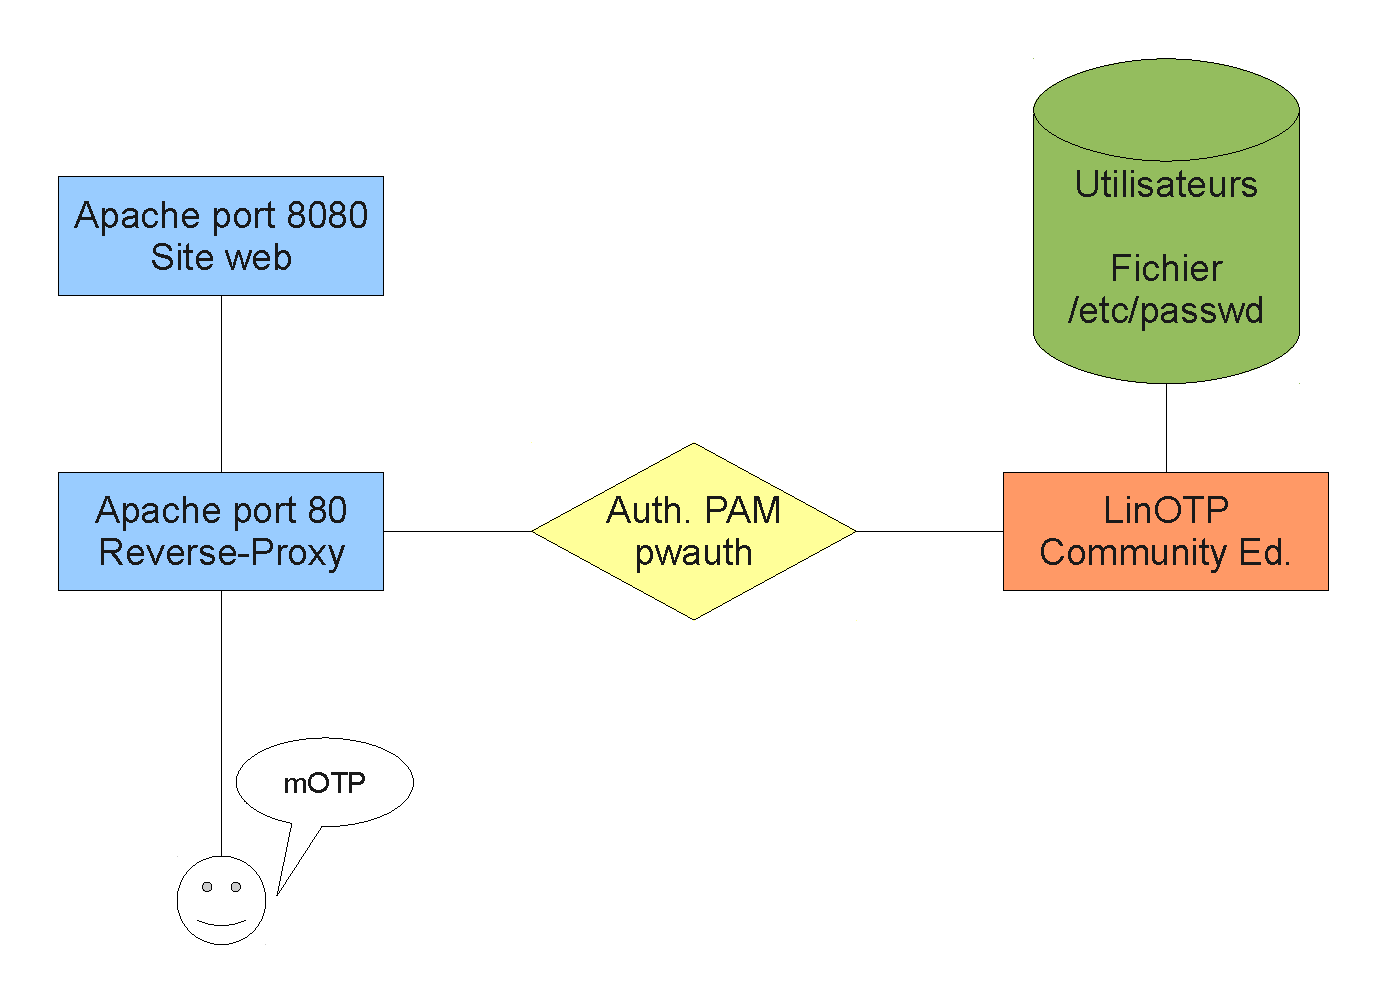
\includegraphics[width=12cm]{linotp/archi-proto}
	\caption{Architecture du prototype \alinotp}
	\label{figure:linotp:archi-proto}
\end{figure}

\paragraph{Architecture}
L'architecture est illustrée en \reffigure{linotp:archi-proto}.
Elle a été mise en place sur un système \alinux{} Debian.

Le portail \aintranet{} \atypo{} est symbolisé par une simple page web hébergée sur un serveur HTTP Apache.
Elle est accessible depuis l'intérieur du réseau \aintranet{} sur le port 8080.
Ce port n'est pas accessible depuis l'extérieur.

Au contraire, le port 80 du serveur Apache peut être contacté depuis \ainternet.
Un \arp{} est alors configuré : l'intérêt est de faire passer l'utilisateur par intermédiaire de ce serveur HTTP pour accéder à la page accessible en interne sur le port 8080.
Celle-ci reste donc toujours isolée de l'extérieur.

Une authentification HTTP Basic\footnote{Dans le cadre d'une transaction HTTP, l'authentification Basic est une méthode permettant de fournir un identifiant et un mot de passe lors d'une requête. Ce couple est fourni via les en-têtes de la requête HTTP.~\cite{httpbasic}} est mise en place sur ce \arp{}.
Quand l'utilisateur a entré son identifiant et son mot de passe issu d'un OTP, le module Apache \amodpam{} prend le relais et réalise une authentification PAM\footnote{Pluggable Authentication Modules (en abrégé PAM) est un mécanisme permettant d'intégrer différents schémas d'authentification de bas niveau dans une API de haut niveau, permettant de ce fait de rendre indépendants du schéma les logiciels réclamant une authentification. PAM est une création de Sun Microsystems et est supporté en 2006 sur les architectures Solaris, \alinux, FreeBSD, NetBSD, AIX et HP-UX.~\cite{pam}}.
Ainsi, on filtre les utilisateurs de façon à ce que seuls ceux qui ont été acceptés par \alinotp{} puissent rentrer.

En effet, un serveur \alinotp{} Community Edition est mis en place, car nous ne disposions pas encore des licences pour la version Enterprise.
Une entrée PAM du système -- contactée par \amodpam{} -- est configurée pour utiliser le module PAM de \alinotp.
En outre, la base d'utilisateurs est simplement représentée par le fichier \texttt{/etc/passwd} du système \alinux. 

Enfin, les utilisateurs utilisent un client \amotp{}\footnote{e.g. DroidOTP sur un téléphone Android} sur leur smartphone pour générer leurs OTP : nous n'avions pas non plus de vrais tokens OTP à notre disposition.

\paragraph{Scénario d'utilisation}
L'authentification sur le prototype avec un client \amotp{} se déroule de la façon suivante :

\begin{enumerate}
	\item l'utilisateur contacte le \arp{} depuis \ainternet{} sur le port 80 grâce à son navigateur web ;
	\item une authentification HTTP de type Basic est demandée à l'utilisateur sur son navigateur ;
	\item l'utilisateur rentre son PIN \amotp{} personnel dans l'application \amotp{} sur son smartphone ;
	\item il obtient alors un OTP qui, précédé par son PIN OTP personnel, forme son mot de passe ;
	\item l'utilisateur s'authentifie dans son navigateur grâce à son identifiant et son mot de passe ;
	\item le \arp{} valide l'authentification, émet une requête HTTP sur le port 8080 pour récupérer la page web en interne ;
	\item le \arp{} retourne la page web a l'utilisateur qui la visualise dans son navigateur web.
\end{enumerate}


\section{Architecture mise en place}
\label{section:linotp:archi-finale}

\begin{figure}
	\centering
	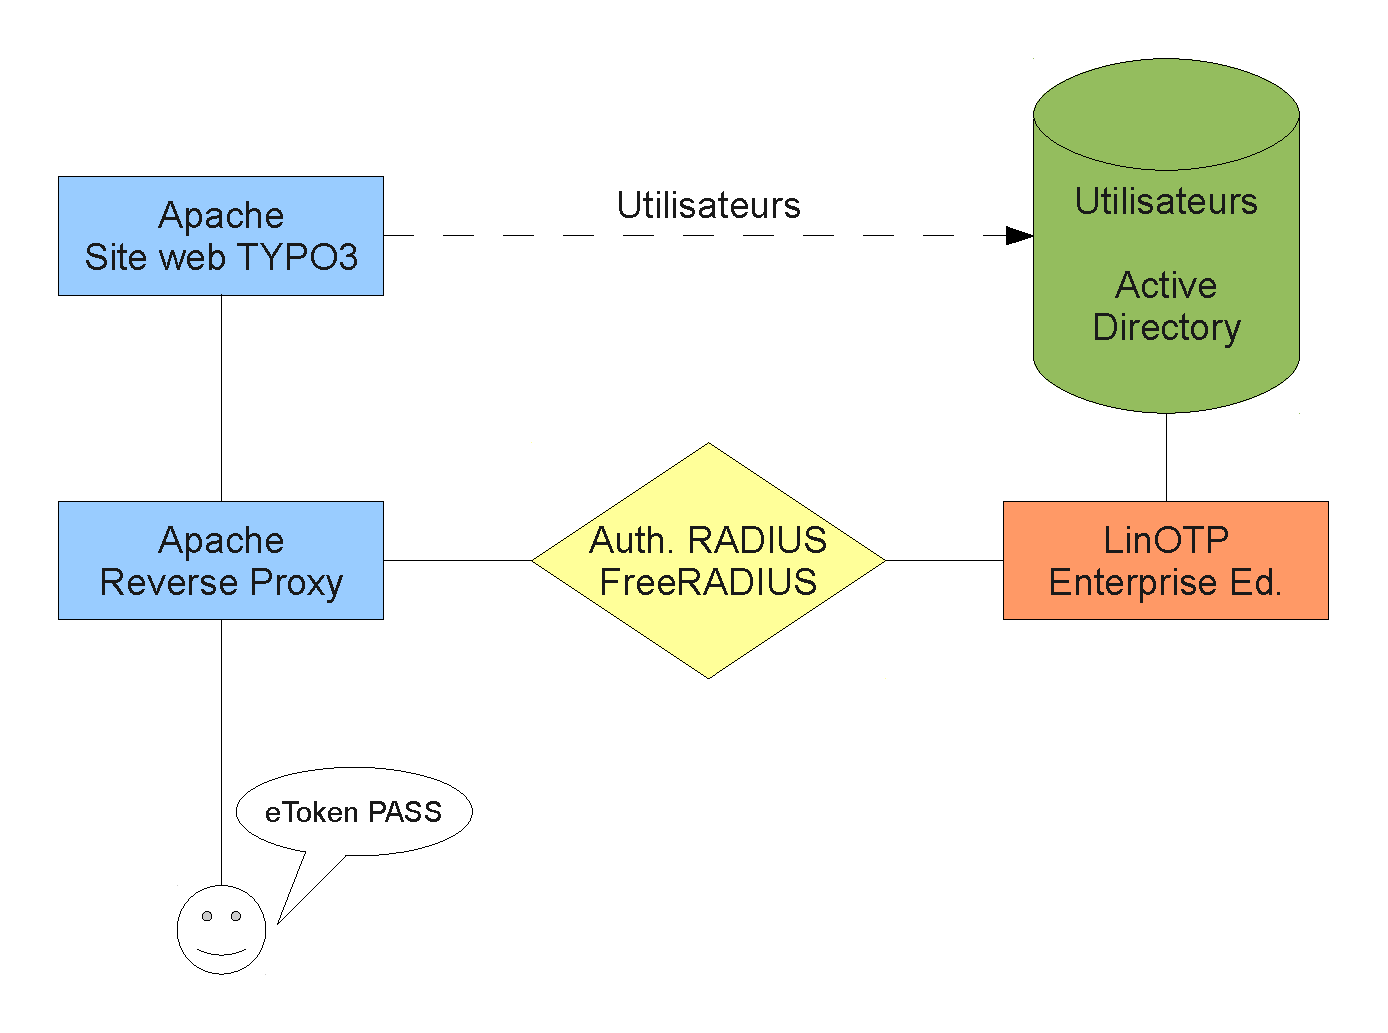
\includegraphics[width=12cm]{linotp/archi-finale}
	\caption{Architecture finale du système d'authentification OTP de la CNIL}
	\label{figure:linotp:archi-finale}
\end{figure}

\paragraph{Architecture}
L'architecture finale est illustrée en \reffigure{linotp:archi-finale}.

Le portail \aintranet{} \atypo{} reste hébergé sur son serveur Apache d'origine, qui n'est accessible que depuis le réseau interne de la CNIL.
Il conserve sa base d'utilisateurs existante qui est liée à l'annuaire \aad{}.

Un autre serveur Apache est mis en place.
Comme dans le prototype, il est configuré en tant que \arp{} pour être l'intermédiaire entre le serveur web du portail et le navigateur de l'utilisateur qui se connecte depuis \ainternet{}.
L'accès est ici aussi filtré par une authentification HTTP Basic.

Par contre, le module d'authentification pour Apache à appeler est dorénavant \amodradius{} : en tant que client \aradius{}, il se charge d'effectuer une requête sur un serveur \afreerad{}\footnote{\afreerad{} est un serveur \aradius{} libre.~\cite{freeradius}} mis en place et configuré spécialement pour ce cas d'utilisation. 
En effet, dans l'architecture finale, on a préféré une authentification via le protocole \aradius{}\footnote{\aradius{} (\etranger{Remote Authentication Dial-In User Service}) est un protocole client-serveur permettant de centraliser des données d'authentification.~\cite{radius}} plutôt que par PAM pour plusieurs raisons :

\begin{itemize}
	\item un serveur \aradius{} est indépendant du système sur lequel il est hébergé, contrairement à PAM ;
	\item le module \amodradius{} pour Apache donne un degré de configuration bien plus intéressant, en permettant entre autres de spécifier la durée de la session de l'utilisateur.
\end{itemize}

En outre, un serveur \alinotp{} Enterprise Edition est mis en place : cette version permet de supporter la connectivité avec le serveur \aradius{} et de résoudre les utilisateurs depuis l'annuaire \aad{} de la CNIL.
D'ailleurs, le serveur \afreerad{} a été compilé avec un module fourni par cette version Enterprise de \alinotp{}, ce qui permet aux deux services de communiquer entre eux.

Enfin, les utilisateurs peuvent cette fois utiliser les tokens Aladdin eToken PASS envoyés par l'éditeur \alse{} pour générer leurs OTP.

\paragraph{Intégration avec l'infrastructure du client}

\begin{figure}
	\centering
	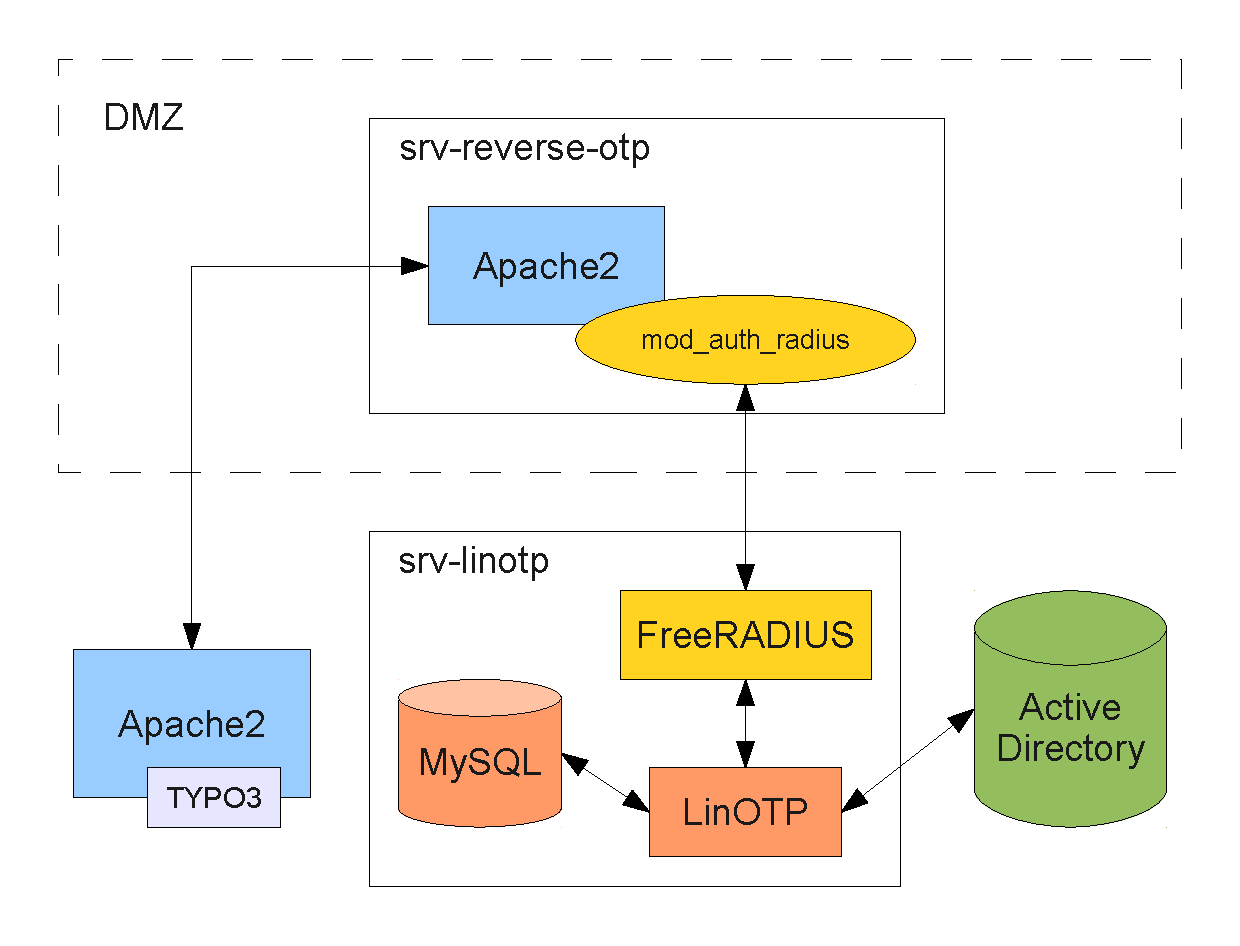
\includegraphics[width=11cm]{linotp/archi-infra}
	\caption{Intégration de la solution \alinotp{} dans l'infrastructure de la CNIL}
	\label{figure:linotp:archi-infra}
\end{figure}

Lors de la mise en place de la solution, il a fallu s'adapter et s'intégrer à l'infrastructure existante du client.
La principale contrainte technique était de monter l'architecture sur des serveurs virtualisés \alinux{} \aredhat{}.
Dans ce contexte, on a l'avantage de pouvoir utiliser autant de machines virtuelles que l'on veut car celles-ci peuvent être créées rapidement et sans coût supplémentaire significatif.

J'ai alors demandé à \amimiette{} de mettre en place deux serveurs virtualisés \aredhat{} :
\begin{itemize}
	\item le premier, \asrvotp{}, localisé dans le réseau interne et hébergeant les services \alinotp{} et \afreerad{} ;
	\item le second, \asrvrp, localisé dans une DMZ\footnote{Une zone démilitarisée (ou DMZ, de l'anglais \etranger{demilitarized zone}) est un sous-réseau isolé du réseau local par un pare-feu. Ce sous-réseau contient les machines étant susceptibles d'être accédées depuis \ainternet.~\cite{dmz}} et donc accessible depuis l'extérieur, qui héberge le \arp{}.
\end{itemize}

Ce partitionnement des services sur deux serveurs différents permet de sécuriser l'architecture.
En effet, seul le \arp{} doit être accessible de l'extérieur.
Si par exemple un pirate arrive à compromettre ce serveur web, le serveur \alinotp{} ainsi que toutes les données qui y sont relatives comme la liste des utilisateurs, les tokens qui leur sont affectés et leurs PIN correspondants ne seront pas mis en danger, à condition que la frontière entre la DMZ et le réseau interne soit suffisamment sécurisée et étanche.

Cette intégration est décrite sur la \reffigure{linotp:archi-infra}.

\paragraph{Scénario d'utilisation}

L'authentification avec un token se déroule de la façon suivante :

\begin{enumerate}
	\item l'utilisateur contacte le \arp{} depuis \ainternet{} grâce à son navigateur web ;
	\item une authentification HTTP de type Basic est demandée à l'utilisateur sur son navigateur ;
	\item l'utilisateur appuie sur le bouton du token ce qui déclenche la génération de l'OTP et son affichage sur l'écran du token ;
	\item l'OTP obtenu précédé par le PIN OTP personnel de l'utilisateur forme son mot de passe ;
	\item l'utilisateur s'authentifie dans son navigateur grâce à son identifiant et son mot de passe ;
	\item le \arp{} valide l'authentification, émet une requête HTTP vers le serveur web hébergeant le portail \atypo{} et récupère la page web demandée ;
	\item le \arp{} retourne la page web a l'utilisateur qui la visualise dans son navigateur web.
\end{enumerate}


\section{Bilan}

Cette prestation a été un succès.
En effet, le client est content du système mis en place.

Pour ma part, j'ai beaucoup appris de cette mission, tant du plan technique que relationnel.
J'ai également eu l'opportunité de me charger d'une partie de la gestion de projet en contactant divers interlocuteurs et en planifiant des rendez-vous.


\chapter{Mise en place d'une solution \acentreon{}}
\label{section:centreon}

\section{La solution \acentreon}

\paragraph{}
\acentreon{} est une plateforme open source de supervision, c'est-à-dire de surveillance du bon fonctionnement d'une infrastructure système.

\paragraph{Principe de la supervision}
De façon classique, on surveille toutes les informations relatives au matériel (température, pannes\ldots) et au système (charge serveur, utilisation de la mémoire et du processeur\ldots) des serveurs d'un parc.
Généralement, on supervise également tous les services applicatifs (serveurs web, serveurs FTP, serveurs de base de données\ldots) qui y sont hébergées.

Ainsi, les administrateurs système peuvent savoir en temps réel quels sont les services et les machines qui sont fonctionnels ou hors-service.
Très souvent, des alertes leurs sont envoyées pour les prévenir d'une rupture de service.
Ces alertes peuvent prendre la forme d'e-mails mais aussi de SMS ou de messages envoyés par messagerie instantanée.

\paragraph{\anagios}
La solution \acentreon{} repose sur \anagios{} pour effectuer toutes les opérations de surveillance, de reporting et de d'alerte.
Par défaut, \anagios{} propose un certain nombre de possibilités que ce soit pour superviser les ressources des serveurs, les services actifs en consultant un port\footnote{Correspondant à la couche de transport du modèle OSI, la notion de port logiciel permet, sur un ordinateur donné, de distinguer différents interlocuteurs. Ces interlocuteurs sont des programmes informatiques qui, selon les cas, écoutent ou émettent des informations sur ces ports. Un port est distingué par son numéro.~\cite{port}} donné ou en interrogeant les machines via le protocole SNMP\footnote{SNMP (pour \etranger{Simple Network Management Protocol}) est un protocole de communication qui permet aux administrateurs réseau de gérer les équipements du réseau, de superviser et de diagnostiquer des problèmes réseaux et matériels à distance.~\cite{snmp}}.

Les possibilités de supervision sont infinies car \anagios{} est doté d'un système de plugins très efficace.
En effet, ces plugins sont de simples programmes exécutables via la ligne de commande, auxquels on passe en paramètre des options de configuration et qui retournent un entier.
On peut donc les développer dans n'importe quel langage de programmation.
C'est la valeur du code retour qui précise si le test effectué par le plugin est passé ou non :

\begin{description}
	\item[0 OK] le test est passé ;
	\item[1 WARNING] le seuil d'alerte est dépassé ;
	\item[2 CRITICAL] le service a un problème ;
	\item[3 UNKNOWN] il est impossible de connaître l'état du service.
\end{description}

Ces différents niveaux, en plus de permettre le déclenchement d'alertes, sont facilement distinguables sur l'interface web de \anagios{} via un code couleur (\cffigure{centreon:nagios}).

Enfin, il est possible de lancer des actions de surveillance à distance via le protocole NRPE (\etranger{Nagios Remote Plugin Executor}).
En effet, celui-ci permet de lancer n'importe quel plugin \anagios{}, si celui-ci est bien installé sur la machine interrogée.
Les informations transitent entre le serveur \anagios{} et les machines surveillées via un tunnel SSL\footnote{SSL (pour \etranger{Secure Sockets Layer}) est un protocole de sécurisation des échanges sur Internet.~\cite{tls}} sécurisé.

\begin{figure}
	\centering
	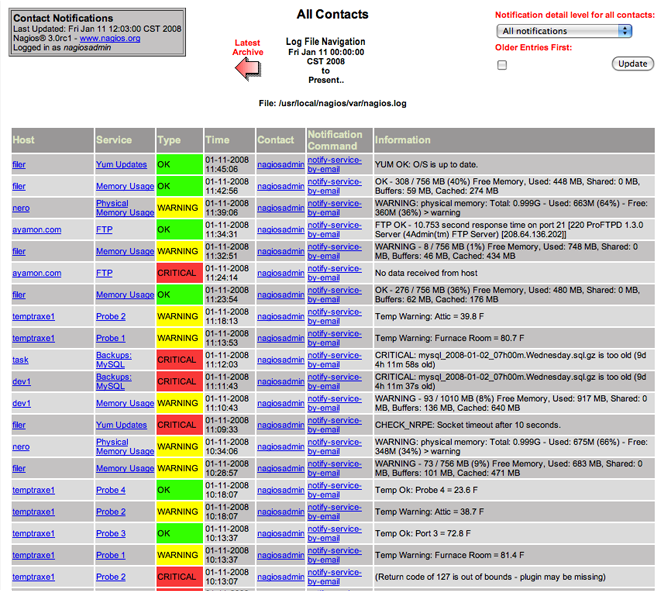
\includegraphics[width=12cm]{centreon/nagios-notifications}
	\caption{Historique des notifications sur Nagios}
	\label{figure:centreon:nagios}
\end{figure}

\paragraph{\acentreon}
Le principal avantage de ce complément à \anagios{} est de fournir une interface graphique web efficace, claire et plus simple à appréhender (\cffigure{centreon:centreon}).

Il ajoute entre autres une gestion fine des utilisateurs, des plugins \anagios{} supplémentaires, des représentations graphiques élaborées, des possibilités d'architecture distribuée, etc.

\begin{figure}
	\centering
	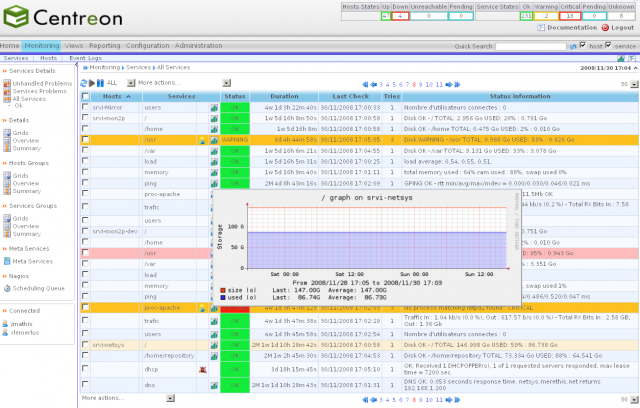
\includegraphics[width=12cm]{centreon/centreon-status}
	\caption{État en temps réel des services sur \acentreon{}}
	\label{figure:centreon:centreon}
\end{figure}


\section{Contexte de la mission}

\paragraph{}
Le client de \asmile{} pour cette mission était \adacast.
C'est une relativement jeune startup présente en France et aux États-Unis.
Son concept est de fournir une plateforme de diffusion multimédia à la demande, en live ou non, performante et simple à utiliser.
Ainsi, ses clients fournissent leurs flux audio ou vidéo et c'est \adacast{} qui se charge de les transformer dans le bon format et les diffuser tout en supportant les éventuels pics d'audience.
\adacast{} propose également différentes façon de monétiser les diffusions, que ce soit par la publicité, par un paiement à la vue ou au forfait.

\paragraph{}
Dans ce contexte, \adacast{} souhaite s'équiper d'une solution de supervision pour surveiller en temps réel son parc de serveurs.
En effet, jusqu'ici, les vérifications de disponibilité de ses services étaient relativement primaires alors que son offre, son nombre de clients et ses enjeux deviennent de plus en plus importants.
Toute rupture de service devient vite critique et doit être prise en charge dans les plus brefs délais.
Il s'agit aussi pour \adacast{} de faire preuve de professionnalisme envers ses clients en dépannant les problèmes avant de recevoir tout coup de fil de plainte.

\paragraph{}
Chez \asmile{}, \asegir{} est le spécialiste de la solution de supervision \acentreon{}.
Je l'ai donc suivi lors de son intervention chez \adacast{} pour apprendre à maîtriser cette technologie.
Nous avons travaillé ensemble la première journée durant laquelle il m'a formé, et j'ai pu terminer la mission seul le lendemain.
\asegir{} est ensuite intervenu à nouveau pour fournir une documentation et former les utilisateurs.


\section{Notre démarche}

\paragraph{}
Pour réduire les coûts et limiter le temps d'intervention, \adacast{} n'a commandé que l'installation de la solution \acentreon{} et la supervision de deux serveurs.
La supervision des autres serveurs serait alors effectuée par ses ressources internes.

\paragraph{}
Pour installer la plateforme \acentreon{}, nous avons demandé à notre interlocuteur de nous fournir un serveur indépendant.
En effet, il est important que la solution de supervision soit sur un serveur qui soit indépendant des serveurs à surveiller.
L'intérêt est à la fois de séparer les services et de ne pas être soumis aux même pannes que ce qui doit être supervisé.

Le client a choisi de commander un serveur à bas coût -- de l'ordre de 20\euro~HT par mois -- chez un hébergeur externe.
Une telle configuration minimaliste est suffisante pour le besoin car peu d'utilisateurs vont consulter la plateforme \acentreon{} et le trafic relatif à l'échange de données de surveillance est limité.

\asegir{} m'a alors montré comment installer \acentreon{} sur un système \alinux{} Ubuntu Server.

\paragraph{}
Nous sommes ensuite passés à la partie la plus intéressante de l'intervention, c'est-à-dire la configuration de la solution en fonction des besoins du client.
Pour cela, des démons NRPE ont été installés sur chaque serveur à superviser.
Nous avons alors mis en place un certain nombre de plugins pour couvrir le périmètre attendu, qui inclut entre autres :

\begin{itemize}
	\item la surveillance des ressources des machines (consommation processeur et mémoire, charge serveur, espace disque disponible) ;
	\item le fonctionnement du RAID matériel ;
	\item la surveillance de la disponibilité de ses services (HTTP, MySQL, FTP, SSH, etc.) ;
	\item la surveillance des métriques relatives à l'utilisation de leur base de données MySQL.
\end{itemize}

\paragraph{}
Enfin, une vue d'ensemble de l'architecture mise en place est illustrée en \reffigure{centreon:archi}.

\begin{figure}
	\centering
	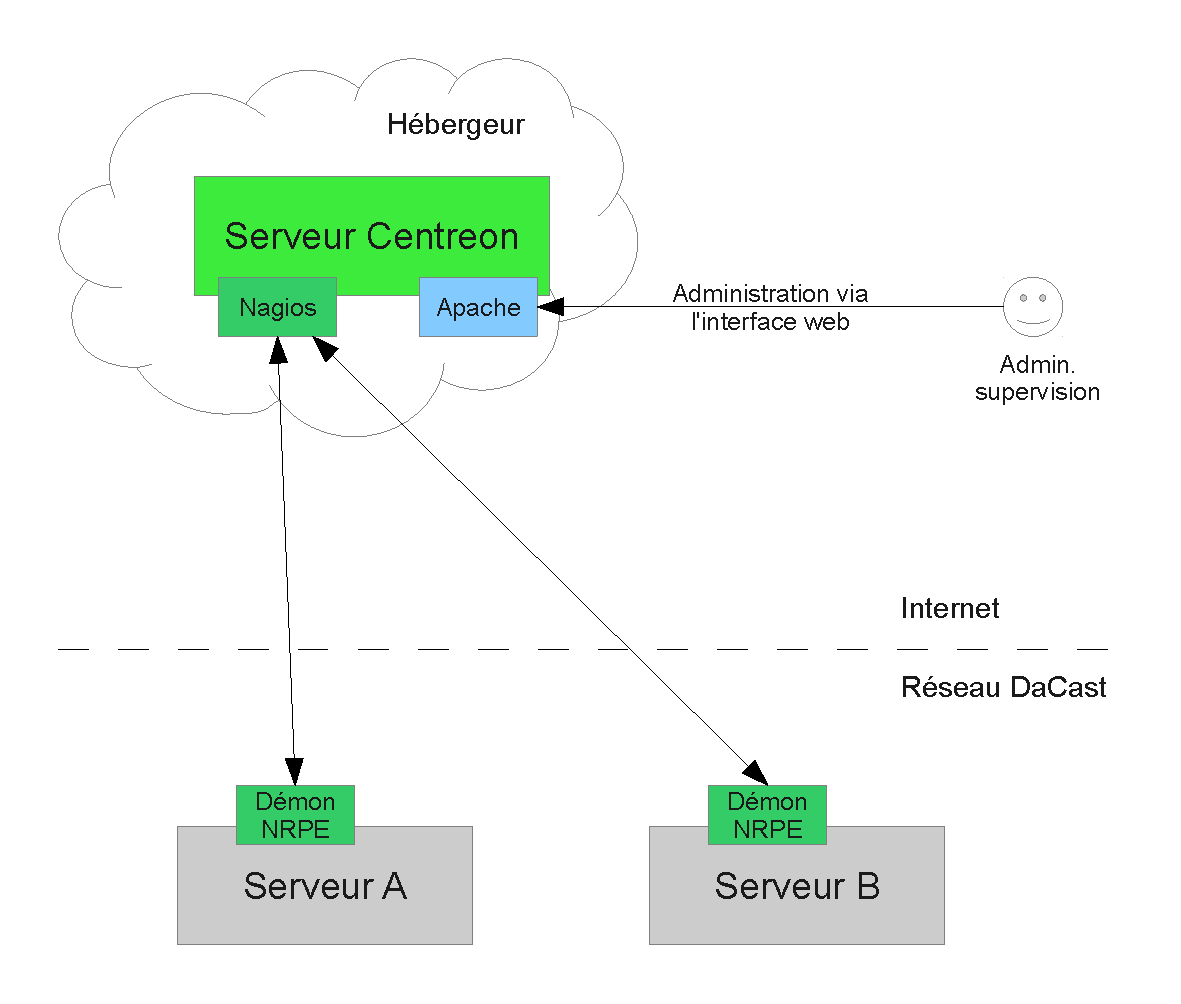
\includegraphics[width=12cm]{centreon/archi}
	\caption{Architecture de supervision mise en place chez \adacast{}}
	\label{figure:centreon:archi}
\end{figure}


\section{Le support projet}

TODO


\chapter{Conclusion}

TODO


\newpage

\bibliographystyle{plain}
\addcontentsline{toc}{chapter}{Bibliographie}
\bibliography{biblio}
\newpage

\appendix

TODO



\end{document}

